%% tex/nondeterminism.tex
%% Copyright 2019 Andrea Berlingieri
%
% This work may be distributed and/or modified under the
% conditions of the LaTeX Project Public License, either version 1.3
% of this license or (at your option) any later version.
% The latest version of this license is in
%   http://www.latex-project.org/lppl.txt
% and version 1.3 or later is part of all distributions of LaTeX
% version 2005/12/01 or later.
%
% This work has the LPPL maintenance status `maintained'.
%
% The Current Maintainer of this work is Andrea Berlingieri.
%
% This work consists of all files listed in manifest.txt
\chapter{Complessita' non deterministica}

\section{Macchine di Turing non deterministiche}

Vediamo un altro modello di calcolo interessante, quello delle Macchine di Turing non
deterministiche.

Una MdT non deterministica e' definita in modo analogo alla versione deterministica, con la sola
differenza che la funzione di transizione $\delta$ e' multivalore:
\begin{equation*}
    \delta \subseteq Q \times \Sigma^{k} \times Q \times (\Sigma \times \set{L,R}^{k})^{k}
\end{equation*}

In altri termini nella MdTN invece di avere una sola quintupla per ogni coppia stato-carattere ne
abbiamo un insieme finito. In un certo senso e' come se avessimo un programma che, invece di avere
una singola istruzione con cui continuare, ha un insieme finito di istruzioni tra cui scegliere per
proseguire la sua computazione.

E' semplice da definire formalmente, basta modificare la definizione della macchina deterministica.
La macchina deterministica e' in un certo senso piu' difficile da definire formalmente rispetto alla
versione non deterministica, dato che la si puo' definire ponendo dei vincoli alla definizione di
quest'ultima.

La macchina deterministica rappresenta un caso particolare della macchina non deterministica dove la
scelta della quintupla e' univoca. Se qualcosa e' calcolabile da una macchina deterministica lo e'
anche da una non deterministica. Di conseguenza le classi deterministiche sono contenute nelle
corripondenti classi non determistiche. Ad esempio, $\PClass \in \NPClass$, $\PSPACE \in \NPSPACE$,
etc.

Definire la MdTN e' semplice. E' piu' complicato definire cosa calcola la MdTN. In una MdTN e'
facile capire che ci sono piu' computazioni possibili. Quale sia pero' il risultato calcolato dalla
macchina non e' ovvio.

Noi ci restringiamo a considerare solamente macchine decisionali, ovvero che rispondono si'/no.
Queste ci sono sufficienti perche' siamo interessati a riconoscere linguaggi. Le nostre macchine
terminano con risposta booleana.

Quando possiamo affermare che una stringa e' accettata da una MdTN? Abbiamo due criteri. Una stringa
puo' essere accettata dalla MdTN se, qualunque computazione della macchina venga fatta, la stringa
viene sempre accettata, oppure puo' essere accettata se esiste una computazione che accetta la
stringa. A noi interessa la seconda definizione, quella della ``macchina fortunata'': ogni volta che
abbiamo una scelta la nostra macchina fa quella giusta.

%Se esiste una computazione della MdTN che porta al riconoscimento la stringa e' considerata
%riconosciuta. // Ripetizione

La computazione della macchina puo' essere rappresentata da un grafo.

\begin{figure}[h]
    \begin{center}
        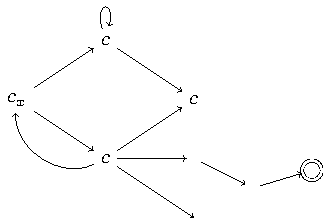
\includegraphics{./img/nondeterminism/MdTN.pdf}    
        \caption{Grafo delle computazioni di una MdTN}
    \end{center}
\end{figure}

Il grafo e' diretto non necessariamente aciclico. Il numero di scelte e' finito e definito dalla
macchina (dal programma), che e' finita. Il grafo non e' neanche necessariamente finito, dato che
possono esistere computazioni che non terminano non cicliche.

Ci porremo piu' avanti il problema di simulare la MdTN, e qui ci tornera' utile questo grafo, detto
grafo delle computazioni.

Alcuni cammini nel grafo portano a stati finali accettanti, altri no, altri possono andare avanti
indefinitamente. A noi basta che esista un cammino che porti ad una configurazione di accettazione
per riconoscere una stringa. 

%La nostra definizione di accettazione ci permettera' di avere delle relazioni con l'esistenza di un
%certificato.

Consideriamo $\SAT$. Come funzionerebbe la MdTN per $\SAT$? Noi dobbiamo prendere una formula
proposizionale e decidere se questa e' soddisfacibile. La nostra macchina comincia a leggere la
formula e trova come prima variabile proposizionale, ad esempio, $A$. $A$ e' vera o falsa? La
macchina ``tira una moneta'' e decide il valore di verita' di $A$. Dopodiche' la macchina va avanti.
Questo processo continua fino alla fine della formula. Se la formula e' soddisfacibile esiste almeno
una computazione fortunata che indovinera' l'assegnazione giusta di valori di verita' alle variabili
proposizionali.

Alla macchina non deterministica basta una scansione lineare della formula, e quindi riesce a
risolvere $\SAT$ in tempo lineare, a patto di prendere la strada giusta. $\SAT$ e' risolvibile in
tempo polinomiale non deterministico da una MdTN. Questa sara' anche il modo in cui definiremo la
classe $\NPClass$.

\section{Complessita' non deterministica}

Dobbiamo definire quali sono il tempo e lo spazio consumati dalla MdTN durante una computazione. Se
la macchina accetta l'input esiste una computazione accettante. Se la risorsa che consideriamo e' il
tempo noi prendiamo il tempo della computazione accettante piu' corta. In termini del grafo delle
computazioni prendiamo il piu' corto cammino accettante della MdTN e la lunghezza di quel cammino e'
il numero di passi richiesto per riconoscere una stringa $x$. Questo numero rappresenta quindi il
tempo richiesto dalla macchina. Indichiamo il tempo richiesto dalla MdTN $M$ su input $x$ con
$\textit{time}_{M}(x)$.

Analogamente per lo spazio prendiamo lo spazio minimo tra gli spazi richiesti dalle computazioni
accettanti. Tuttavia bisogna fare attenzione al come calcoliamo lo spazio richiesto da una
computazione. Questo corrisponde al massimo spazio usato in una configurazione della computazione.
Dobbiamo considerare il ``minimo dei massimi''. Indichiamo lo spazio richiesto dalla MdTN $M$ su
input $x$ con $\textit{space}_{M}(x)$.

Le funzioni $t_{M}$ e $s_{M}$ sono definite identicamente a come lo erano nel caso deterministico, a
patto di usare le nozioni di $\textit{time}$ e $\textit{space}$ appena definite. Un discorso analogo
di applica alle definizioni di $\NTIME(f)$ e $\NSPACE(f)$.

Possiamo definire le classi $\NPClass$, $\NEXP$, $\NLOGSPACE$ e $\NPSPACE$ in maniera identica a
come abbiamo definito le corrispondenti classi deterministiche, avendo cura di usare $\NTIME$ al
posto di $\DTIME$ e analogamente per lo spazio.

Possiamo formalizzare quanto detto prima sulla relazione tra macchine di Turing deterministiche e
non deterministiche con il seguente teorema.
\begin{thm}
    Per ogni $f: \Nat \to \Nat$
    \begin{equation*}
        \DTIME(f) \subseteq \NTIME(f) \land \DSPACE(f) \subseteq \NSPACE(f)
    \end{equation*}
\end{thm}
La dimostrazione e' ovvia essendo la macchina di Turing determinstica un caso particolare della
macchina non deterministica.

%(Abbiamo saltato la riduzione dei nastri)

\section{Simulazione del non determinismo}

Vogliamo stabilire delle relazioni tra la MdTN e la corrispondente macchina deterministica. Per
stabilire queste relazioni una tecnica che risulta utile e' pensare in termini di simulazione.
Siamo quindi interessati a teoremi che riguardano la simulazione del nondeterminismo.

Immaginiamo di avere una macchina non deterministica che riconosce un linguaggio con una certa
complessita' e immaginiamo di simularla con una macchina deterministica. Se riusciamo a determinare
la complessita' della simulazione rispetto alla complessita' della macchina di partenza riusciamo a
dire qualcosa sulla complessita' del riconoscimento del linguaggio in modo deterministico.

C'e' un modo interessante di vedere la simulazione della MdTN: consideriamo il grafo delle
computazioni di una MdTN. Per simulare la macchina in modo deterministico ci basta trovare un
algoritmo deterministico di visita dei cammini del grafo. Dobbiamo fare un'esplorazione completa,
dato che possono esistere in generale cammini di riconoscimento migliori di uno gia' trovato.
Dobbiamo fare una qualche visita astuta per effettuare la simulazione.

%Slide 89

In generale quando vogliamo stabilire delle relazioni tra classi deterministiche e classi non
deterministiche usiamo classi di risorse diverse. Ad esempio, avendo un bound di tempo alla
complessita' della MdTN diciamo qualcosa riguardo alla complessita' in spazio della simulazione
deterministica. Il primo teorema che vediamo mostra questo.

Supponiamo di conoscere la complessita' $O(f)$ in tempo della macchina non deterministica e ci
chiediamo quale sia la complessita' in spazio della simulazione deterministica, cercando di
minimizzare l'occupazione di memoria.

Quello che dobbiamo fare e' occupare il minor spazio possibile durante la nostra visita del grafo
delle computazioni. La visita in ampiezza non e' la migliore scelta in questo caso, dato che in
generale potremmo avere una frontiera attiva dei nodi da visitare molto ampia che non ci e'
necessaria.

Abbiamo che la MdTN lavora in $\NTIME(f)$. Abbiamo che $f$ rappresenta la lunghezza massima dei
cammini da esplorare, dato che sappiamo che nostra macchina non deterministica riconosce il nostro
linguaggio in tempo $O(f)$. Rispetto a questa lunghezza dei cammini il numero di nodi che possiamo
avere cresce in generale esponenzialmente: se avessimo, ad esempio, per ogni nodo, una scelta
binaria avremmo $2^{n}$ nodi.

Consideriamo una visita in profondita'. Esploriamo il primo cammino, con lunghezza $O(f(|x|))$.
Quante configurazioni incontriamo? $O(f(|x|))$. Possiamo dire qualcosa sulla dimensione di queste
configurazioni? 

Abbiamo che anche per la MdTN il tempo fa da bound al tempo. Per ogni configurazione l'aspetto che
influisce di piu' sull'occupazione di spazio e' la dimensione dei nastri. I nastri crescono, al
massimo, in modo lineare rispetto al tempo. La dimensione dei nastri e' bound da $O(f(|x|))$. Per
memorizzare la catena della configurazioni ci serve $O((f(|x|))^{2})$ spazio. 

Questo e' lo spazio richiesto per la visita di un ramo del grafo. Tuttavia il ramo che stiamo
visitando potrebbe essere un ramo di fallimento, oppure un ramo che diverge. Nel caso fossimo in uno
di questi due casi, una volta raggiunta una configurazione di fallimento o una volta che abbiamo
raggiunto il bound in tempo della MdTN senza accettare possiamo tornare indietro lungo il ramo alla
prima configurazione dove ci e' ancora possibile fare una scelta e effettuarne una diversa.
Procediamo quindi per backtracking. In ogni caso l'occupazione di tutti i cammini che esploriamo ha
gli stessi upper bound dati per il primo cammino.

Con una simulazione di questo tipo lo spazio richiesto dalla simulazione deterministica della MdTN
e' dell'ordine di $O(f^{2})$.

Possiamo pero' fare di meglio. Perche'?

In generale come facciamo a risparmiare spazio? Possiamo rendere implicite le rappresentazioni
esplicite dei dati, attraverso una descrizione compatta che prendera' tempo al momento
dell'esecuzione ma ci permettera' di risparmiare spazio. Al costo del tempo risparmiamo spazio.
Tutto cio' che ci e' oneroso dal punto di vista della memoria lo rendiamo implicito attraverso una
sintesi compatta (ad esempio una compressione). Quando, in fase di esecuzione, avremo bisogno del
dato ci bastera' spendere un po' di tempo per estrarlo dalla sua descrizione.

Abbiamo una tecnica analoga per risparmiare tempo a costo dello spazio. Pensiamo ad esempio alla
programmazione dinamica con memoization. Manteniamo una tabela per memorizzare le soluzioni dei
sottoproblemi. Quando ci serve una soluzione ad un sottoproblema possiamo guardare la tabella e, nel
caso il sottoproblema sia gia' stato risolto, ottenere subito il risultato richiesto. Se questo non
e' il caso risolviamo il sottoproblema e memorizziamo la soluzione in tabella per usi futuri.

Tempo e spazio sono due risorse ``complementari''. Non si puo', allo stesso tempo, ottimizzare il
tempo e lo spazio. Ottimizzare in tempo richiede spendere in spazio e viceversa.  Di solito siamo
portati a pensare a ottimizzazioni del tempo, senza considerare lo spazio.

Quello che occupa piu' spazio nella nostra visita dei cammini e' la memorizzazione esplicita della
catena di configurazioni. Possiamo dare una descrizione del cammino che prendiamo nel grafo molto
piu' compatta, ad esempio come sequenza di scelte fatte dalla configurazione iniziale. Possiamo
etichettare ogni scelta nel cammino con un numero e salvarci le etichette del nostro cammino.
L'unica informazione che ci serve per definire il cammino e' la sequenza delle scelte prese. Nel
caso dovessimo fare backtracking possiamo ripercorrere tutte le scelte del cammino corrente fino
alla scelta da rivedere e cambiare scelta. Considerando tutte le possibili scelte avremo considerato
tutti i possibili cammini del grafo.

Quanto ci costa memorizzare questa sequenza di scelte? L'unica configurazione che teniamo attiva e'
quella finale, che e' bound da $O(f(|x|))$ per il teorema tempo spazio. Le scelte sono in un range
finito fissato dalla macchina.

In definitiva ci serviranno $c\cdot O(f(|x|))$ per memorizzare le scelte e $O(f(|x|))$ per la
configurazione finale del cammino. L'ordine dell'occupazione di spazio della simulazione fatta in
questo modo e' quindi $O(f(|x|))$. Riusciamo a fare la simulazione della MdTN in spazio $O(f(x))$.

\begin{thm}
    Per ogni $f:\Nat \to \Nat$ costruibile in spazio maggiore o uguale all'identita'
    \begin{equation*}
        \NTIME(f) \subseteq \DSPACE(f)
    \end{equation*}
\end{thm}

Possiamo vedere la simulazione in un modo piu' operazionale. Dato $x$ inizializziamo due nastri di
dimensione $f(|x|)$. In un nastro memorizziamo il tape e in un altro le scelte. All'inizio
simuleremo la computazione dove la scelta che facciamo e' sempre la prima. Sul nastro del tape
simuliamo la computazione della MdTN. A questo punto arriviamo in fondo in vari modi: o terminiamo
il tempo, o cerchiamo di sforare lo spazio, o ci arrestiamo con riconoscimento, o ci arrestiamo con
fallimento. In quest'ultimo caso andiamo a cambiare l'ultima scelta per fare backtracking e
rifacciamo la computazione. L'occupazione di spazio rimane dell'ordine $O(f)$. Dovremmo memorizzare
anche un timer per non sforare in tempo, ma questo ha occupazione logaritmica nel valore di $f$, di
conseguenza l'occupazione di spazio non peggiora.

\begin{figure}[h]
    \begin{center}
        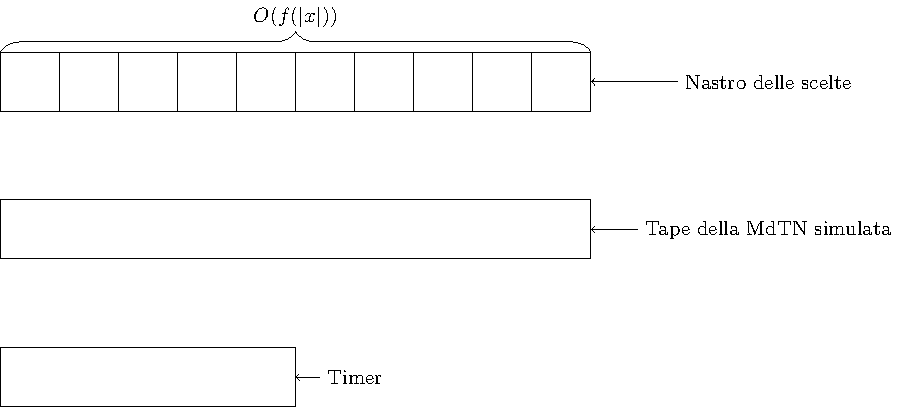
\includegraphics[scale=0.7]{./img/nondeterminism/Simulation.pdf}
        \caption{Simulazione deterministica di una MdTN con memoriazzazione delle scelte}
    \end{center}
\end{figure}
